\begin{center}
	\textbf{{\Huge ĐỀ 004}}
\end{center}
\subsubsection*{Phần I. Thí sinh trả lời từ câu 1 đến câu 12, mỗi câu hỏi chọn một phương án.}
\setcounter{bt}{0}\setlist[enumerate,1]{label=\quad\bfseries\Alph*.}
\begin{baitap}
%	\textbf{Câu 3.} 
	Cho hàm số có đồ thị $y = f(x)$ như hình vẽ bên dưới. Hàm số đã cho nghịch biến trên khoảng nào sau đây?
	
	\begin{minipage}{0.4\textwidth}
		\begin{enumerate}
			\item $(-1; 1)$.
			\item $(-\infty; 1)$.
			\item $(-\infty; -1)$.
			\item $(-1; +\infty)$.
		\end{enumerate}
	\end{minipage}
	\begin{minipage}{0.5\textwidth}
		% Cubic function graph y = -x^3 + 3x with local min at (-1,-2) and local max at (1,2)
		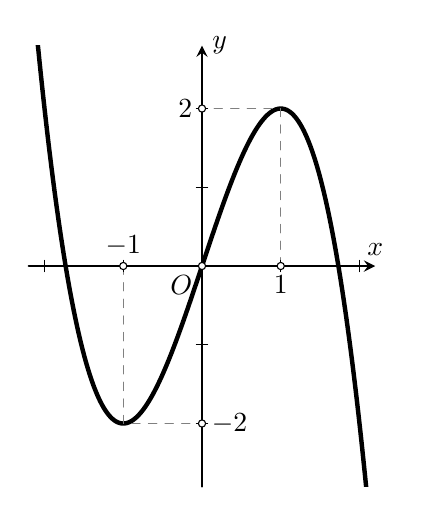
\begin{tikzpicture}[line cap=round, line join=round, >=stealth, scale=1]
			% Window bounds
			\def\xmin{-2.2} \def\xmax{2.2}
			\def\ymin{-2.8} \def\ymax{2.8}
			
			% Scope to clip the curve safely within bounds
			\begin{scope}
				\clip (\xmin,\ymin) rectangle (\xmax,\ymax);
				
				% Graph of y = -x^3 + 3x
				\draw[black, ultra thick, smooth, samples=200, domain=\xmin:\xmax]
				plot(\x, { -1*(\x)^3 + 3*(\x) });
			\end{scope}
			
			% Dashed projection lines for local extrema
			\draw[dashed, gray, thin] (-1,0) -- (-1,-2) -- (0,-2);
			\draw[dashed, gray, thin] (1,0) -- (1,2) -- (0,2);
			
			% Draw Coordinate Axes
			\draw[->, thick] (\xmin,0) -- (\xmax,0) node[above]{$x$};
			\draw[->, thick] (0,\ymin) -- (0,\ymax) node[right]{$y$};
			
			% Tick marks on axes
			\foreach \x in {-2,-1,1,2}
			\draw (\x,2pt) -- (\x,-2pt);
			\foreach \y in {-2,-1,1,2}
			\draw (2pt,\y) -- (-2pt,\y);
			
			% Key points marked with small open circles
			\draw[fill=white] (-1,0) circle (1.3pt);
			\draw[fill=white] (1,0) circle (1.3pt);
			\draw[fill=white] (0,-2) circle (1.3pt);
			\draw[fill=white] (0,2) circle (1.3pt);
			\draw[fill=white] (0,0) circle (1.3pt);
			
			% Axis labels
			\node[below left] at (0,0) {$O$};
			\node[above] at (-1,0) {$-1$};
			\node[below] at (1,0) {$1$};
			\node[left] at (0,2) {$2$};
			\node[right] at (0,-2) {$-2$};
		\end{tikzpicture}
	\end{minipage}
	\begin{traloi}
		\dapan{C}
		Quan sát hình vẽ thấy trên khoảng $ (-\infty;-1) $ đồ thị hàm số hướng đi xuống, nên hàm số nghịch biến trên khoảng đó.
	\end{traloi}
\end{baitap}

\begin{baitap}
	Cho hàm số $y = f(x)$ liên tục trên $\mathbb{R}$ và có đạo hàm là $f'(x) = x^2 (x^2 - 5x + 4)$, $\forall x \in \mathbb{R}$. Hàm số $f(x)$ có bao nhiêu điểm cực tiểu?
	\begin{multicols}{4}
		\begin{enumerate}
			\item $0$.
			\item $2$.
			\item $1$.
			\item $3$.
		\end{enumerate}
	\end{multicols}
	\begin{traloi}
		\dapan{C}
		Giải phương trình $ f'(x)=0 $ tìm được các nghiệm $ 0,1.4 $ nên lập được bảng biến thiên sau:
		\begin{center}
			
\begin{tikzpicture}
				\tkzTabInit[lgt=1.2, espcl=2.5]{$x$/1,$y'$/1,$y$/1.5}
				{
					$-\infty$,$ 0 $, $ 1 $,	$4$,$ +\infty $
				}
				\tkzTabLine{,+,z,+,z,-,z,+,}
				\tkzTabVar{-/,R, +/, -/,+/,}
			\end{tikzpicture}
		\end{center}
	\end{traloi}
\end{baitap}

\begin{baitap}
%	\textbf{Câu 5.} 
	Giá trị nhỏ nhất của hàm số $y = \sqrt{16 - x^2}$ trên đoạn $[-2; 2]$ bằng
	\begin{multicols}{4}
		\begin{enumerate}
			\item $4$.
			\item $2\sqrt{3}$.
			\item $2\sqrt{5}$.
			\item $0$.
		\end{enumerate}
	\end{multicols}
	\begin{traloi}
		\dapan{B} Giá trị nhỏ nhất của hàm số trên đoạn $[-2; 2]$ bằng $2\sqrt{3}$. Dưới đây là các bước giải chi tiết:		
		\begin{itemize}
			\item Tập xác định và tính liên tục:  Hàm số $y = \sqrt{16 - x^2}$ xác định và liên tục trên đoạn $[-2; 2]$.
			\item Tính đạo hàm: $y' = \dfrac{-x}{\sqrt{16 - x^2}}$ với $x \in (-2; 2)$.
			\item  $y' = 0 \iff x = 0 \in [-2; 2]$.
			\item Tính giá trị hàm số tại hai điểm mút và điểm tới hạn:
			$$y(-2) = 2\sqrt{3},\quad y(0) =4, \quad y(2) = 2\sqrt{3}$$
			\item Kết luận: $$\min\limits_{[-2; 2]} y = 2\sqrt{3} \quad \text{tại } x = \pm 2$$
		\end{itemize}
	\end{traloi}
\end{baitap}
\begin{baitap}
	%	\textbf{Câu 5.} 
	Giá trị nhỏ nhất của hàm số $y = 2 \cos^3 x - \frac{9}{2} \cos^2 x + 3 \cos x + \frac{1}{2}$ là
	\begin{multicols}{4}
		\begin{enumerate}
			\item $-9$.
			\item $1$.
			\item $-\frac{3}{2}$.
			\item $\frac{1}{2}$.
		\end{enumerate}
	\end{multicols}
	\begin{traloi}
		\dapan{A}  Đặt $t = \cos x$. Vì $-1 \le \cos x \le 1$ nên $t \in [-1; 1]$. 	Bài toán trở thành tìm giá trị nhỏ nhất của hàm số:
		$$f(t) = 2t^3 - \frac{9}{2}t^2 + 3t + \frac{1}{2} \quad \text{trên đoạn } [-1; 1]$$
	\end{traloi}
\end{baitap}

\begin{baitap}
%	\textbf{Câu 10.} 
	Tiếp tuyến của đồ thị hàm số $y = \dfrac{2x + 3}{x - 2}$ tại điểm có hoành độ bằng $3$ có phương trình là
	\begin{multicols}{4}
		\begin{enumerate}
			\item $y = 7x + 13$.
			\item $y = 30 - 7x$.
			\item $y = 3x + 9$.
			\item $y = -\dfrac{4}{3}x - 2$.
		\end{enumerate}
	\end{multicols}
	\begin{traloi}
		\dapan{B} 
		\begin{itemize}
			\item Tính tung độ $y_0$ của tiếp điểm.	Thay $x_0 = 3$ vào hàm số:
		
		$$y_0 = \dfrac{2(3) + 3}{3 - 2} = \dfrac{9}{1} = 9$$
		
		\item Tính đạo hàm $y'$ và hệ số góc $k$ của tiếp tuyến.  $$y' = \dfrac{2(-2) - 3(1)}{(x - 2)^2} = \dfrac{-7}{(x - 2)^2}$$
		
		Suy ra hệ số góc của tiếp tuyến tại $x_0 = 3$ là: $$k = y'(3) = \dfrac{-7}{(3 - 2)^2} = -7$$
		
		\item Viết phương trình tiếp tuyến.  Phương trình tiếp tuyến tại điểm $M(3; 9)$ có dạng:
		
		$$y = k(x - x_0) + y_0$$
		
		Từ đó tìm được phương trình tiếp tuyến của đồ thị hàm số là $y = -7x + 30$.
		\end{itemize}
	\end{traloi}
\end{baitap}

\begin{baitap}
%	\textbf{Câu 11.} 
	Hàm số $y = f(x) = \frac{1}{2}x^2 + x - 6\ln x + 2025$ nghịch biến trên khoảng nào sau đây?
	\begin{multicols}{4}
		\begin{enumerate}
			\item $(-3; 2)$.
			\item $(2; +\infty)$.
			\item $(0; 3)$.
			\item $(0; 1)$.
		\end{enumerate}
	\end{multicols}
	\begin{traloi}
		\dapan{D}
		Điều kiện xác định: $ x>0. $
		Ta có
		\[
		f'(x)=x+1-\frac6x
		=\frac{x^2+x-6}{x}
		=\frac{(x+3)(x-2)}{x}.
		\]
		
		Vì \(x>0\) nên \(x>0\) và \(x+3>0\). Do đó
		\[
		f'(x)<0\iff x-2<0\iff 0<x<2.
		\]
		
		Vậy hàm số nghịch biến trên khoảng $ (0;2) $, do đó chọn đáp án D.
	\end{traloi}
\end{baitap}

\begin{baitap}
%	\textbf{Câu 8.} 
	Tìm giá trị thực của tham số $a$ để hàm số $f(x) = -x^3 - 3x^2 + a$ có giá trị nhỏ nhất trên đoạn $[-1; 1]$ bằng $0$.
	\begin{multicols}{4}
		\begin{enumerate}
			\item $a = 2$.
			\item $a = 6$.
			\item $a = 0$.
			\item $a = 4$.
		\end{enumerate}
	\end{multicols}
	\begin{traloi}
		\dapan{D}
		Xét
		\[
		f(x)=-x^3-3x^2+a,\qquad x\in[-1;1].
		\]
		
		Ta có
		\[
		f'(x)=-3x^2-6x=-3x(x+2).
		\]
		
		Trên \([-1;1]\):
		\[
		f'(x)=0\iff x=0.
		\]
		
		Tính giá trị tại hai đầu mút và điểm tới hạn:
		\[
		f(-1)=a-2,\qquad f(0)=a,\qquad f(1)=a-4.
		\]
		
		Do đó
		\[
		\min_{[-1;1]}f(x)=a-4.
		\]
		
		Theo giả thiết giá trị nhỏ nhất bằng \(0\), nên
		\[
		a-4=0
		\iff \boxed{a=4}.
		\]
	\end{traloi}
\end{baitap}

\begin{baitap}
	%	\textbf{Câu 12.} 
	Một cửa hàng buôn giày nhập một đôi với giá là $40$ đô-la. Cửa hàng ước tính rằng nếu đôi giày được bán với giá $x$ đô-la thì mỗi tháng khách hàng sẽ mua $(120 - x)$ đôi. Hỏi cửa hàng bán một đôi giày giá bao nhiêu đô-la thì thu được nhiều lãi nhất?
	\begin{multicols}{4}
		\begin{enumerate}
			\item $80$.
			\item $160$.
			\item $40$.
			\item $240$.
		\end{enumerate}
	\end{multicols}
	\begin{traloi}
		\dapan{A}
		Lợi nhuận mỗi tháng là
		\[
		P(x)=(x-40)(120-x)=-x^2+160x-4800.
		\]
		Đây là parabol quay xuống, đạt giá trị lớn nhất tại
		\[
		x=-\frac{160}{2(-1)}=80.
		\]
		
		Vậy giá bán để thu được nhiều lãi nhất là
		\[
		\boxed{80\text{ đô-la}}.
		\]
	\end{traloi}
\end{baitap}

\begin{baitap}
%	\textbf{Câu 9.} 
	Cho hàm số $y = f(x)$ liên tục trên $\mathbb{R}$ và có đồ thị như hình bên. 
	
	\begin{minipage}{0.5\textwidth}
		Tìm giá trị lớn nhất của hàm số $y = f^2(x) + 3$ trên đoạn $[0; 2]$.
			\begin{enumerate}
			\item $12$.
			\item $13$.
			\item $2$.
			\item $9$.
		\end{enumerate}
	\end{minipage}
	\begin{minipage}{0.4\textwidth}
		% Cubic function y = x^3 - 3x^2 + 1 with local max (0,1) and local min (2,-3)
		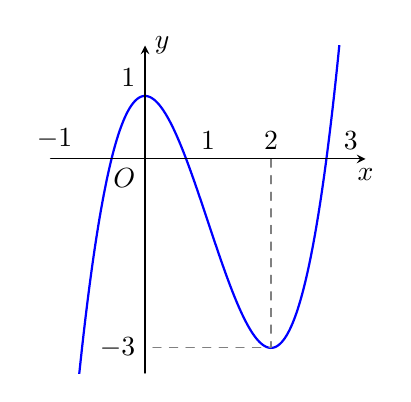
\begin{tikzpicture}[line cap=round, line join=round, >=stealth, scale=.8]
			% Define window bounds
			\def\xmin{-1.5} \def\xmax{3.5}
			\def\ymin{-3.4} \def\ymax{1.8}
			
			% Scope to clip the curve safely within bounds
			\begin{scope}
				\clip (\xmin,\ymin) rectangle (\xmax,\ymax);
				
				% Graph of y = x^3 - 3x^2 + 1
				\draw[blue, thick, smooth, samples=200, domain=\xmin:\xmax]
				plot(\x, {(\x)^3 - 3*(\x)^2 + 1});
			\end{scope}
			
			% Dashed projection lines for local minimum (2, -3)
			\draw[dashed, gray, thin] (2,0) -- (2,-3) -- (0,-3);
			
			% Draw Coordinate Axes
			\draw[->] (\xmin,0) -- (\xmax,0) node[below]{$x$};
			\draw[->] (0,\ymin) -- (0,\ymax) node[right]{$y$};
			
			% Labels for key points and values
			\node[below left] at (0,0) {$O$};
			\node[above left] at (0,1) {$1$};
			\node[above left] at (-1,0) {$-1$};
			\node[above] at (1,0) {$1$};
			\node[above] at (2,0) {$2$};
			\node[above right] at (3,0) {$3$};
			\node[left] at (0,-3) {$-3$};
		\end{tikzpicture}
	\end{minipage}
	\begin{traloi}
		\dapan{A}
		Trên đoạn \([0;2]\), từ đồ thị ta có \(-3\le f(x)\le1\), nên \(\max f^2(x)=9\). Do đó \(\max [f^2(x)+3]=9+3=12\).
	\end{traloi}
\end{baitap}

\begin{baitap}
%	\textbf{Câu 10.} 
	Cho hàm số $f(x) = \dfrac{x - m^2}{x + 8}$ với $m$ là tham số thực. Tìm giá trị lớn nhất của $m$ để hàm số có giá trị nhỏ nhất trên đoạn $[0; 3]$ bằng $-2$.
	\begin{multicols}{4}
		\begin{enumerate}
			\item $m = -4$.
			\item $m = 5$.
			\item $m = 4$.
			\item $m = 1$.
		\end{enumerate}
	\end{multicols}
	\begin{traloi}
		\dapan{C}
		Ta có \(f'(x)=\frac{8+m^2}{(x+8)^2}>0\), nên \(f(x)\) đồng biến trên \([0;3]\). Do đó \(\min_{[0;3]}f(x)=f(0)=-\frac{m^2}{8}=-2\), suy ra \(m^2=16\), nên \(m=\pm4\). Vậy giá trị lớn nhất của \(m\) là \(4\).
	\end{traloi}
\end{baitap}

\begin{baitap}
%	\textbf{Câu 11.} 
	Cho hàm số $f(x)$ có đạo hàm $f'(x) = (x + 1)(x - 1)^2(x - 2)$. Giá trị nhỏ nhất của hàm số $g(x) = f(x) + \frac{1}{3}x^3 - x - 2$ trên đoạn $[-1; 2]$ bằng
	\begin{multicols}{4}
		\begin{enumerate}
			\item $f(2) - \frac{4}{3}$.
			\item $f(1) - \frac{8}{3}$.
			\item $f(0) - 2$.
			\item $f(-1) - \frac{4}{3}$.
		\end{enumerate}
	\end{multicols}
\begin{traloi}
	\dapan{B}
	Ta có \(g'(x)=(x+1)(x-1)(x^2-3x+3)\). Vì \(x^2-3x+3>0\) với mọi \(x\), nên ta có bảng biến thiên:
	\begin{center}
		
\begin{tikzpicture}
			\tkzTabInit[lgt=1.2, espcl=2.5]{$x$/1,$g'(x)$/1,$g(x)$/1.5}
			{
				$-1$,
				$1$,
				$2$
			}
			\tkzTabLine{,-,z,+,}
			\tkzTabVar{+/, -/$ g(1) $, +/}
		\end{tikzpicture}
	\end{center}
	Dựa vào bảng biến thiên ta có hàm số đạt giá trị nhỏ nhất tại \(x=1\):
	\[
	\min_{[-1;2]}g(x)=g(1)=f(1)-\frac83.
	\]
\end{traloi}
\end{baitap}

\begin{baitap}
%	\textbf{Câu 12.} 
	Tập hợp nào dưới đây chứa tất cả các giá trị thực của tham số $m$ để giá trị lớn nhất của hàm số $y = \left|x^4 - 2x^2 + m\right|$ trên đoạn $[0; 2]$ bằng $5$?
	\begin{multicols}{2}
		\begin{enumerate}
			\item $(-\infty; -5) \cup (0; +\infty)$.
			\item $(-5; -2)$.
			\item $(-4; -1) \cup (5; +\infty)$.
			\item $(-4; -3)$.
		\end{enumerate}
	\end{multicols}
	\begin{traloi}
		\dapan{B}
		Đặt \(u=x^4-2x^2\). Trên \([0;2]\), ta có \(\min u=-1\), \(\max u=8\). Do đó $$\max|u+m|=\max\{|m-1|,|m+8|\}=5.$$
		
		Suy ra \(m=-4\) hoặc \(m=-3\). Cả hai giá trị đều thuộc \((-5;-2)\).
	\end{traloi}
\end{baitap}
\enlargethispage{\baselineskip}
\subsubsection*{Phần II. Thí sinh trả lời từ câu 1 đến câu 4, trong ý a), b), c), d) ở mỗi câu câu, thí sinh chọn ĐÚNG hoặc SAI.}
\setcounter{bt}{0}\setlist[enumerate,1]{label=\quad\bfseries\alph*)}
\begin{baitap}
%	\textbf{Câu 1:}BGD 2025 
	Cho hàm số $f(x) = x^3 - 12x - 8$.
	\begin{enumerate}
		\item Hàm số đã cho có đạo hàm là $f'(x) = 3x^2 - 12$.
		\item Phương trình $f'(x) = 0$ có tập nghiệm là $S = \{2\}$.
		\item $f(2) = 24$.
		\item Giá trị lớn nhất của hàm số $f(x)$ trên đoạn $[-3; 3]$ bằng $24$.
	\end{enumerate}
	\begin{traloi}
		\dapan{Đúng -- Sai -- Sai -- Sai}
		\begin{enumerate}
			\item Đúng, vì \(f'(x)=3x^2-12\).
			\item Sai, vì \(f'(x)=0\iff x=\pm2\), nên \(S=\{-2;2\}\).
			\item Sai, vì \(f(2)=8-24-8=-24\).
			\item Sai, vì \(f(-3)=1,\ f(-2)=8,\ f(2)=-24,\ f(3)=-17\). Do đó GTLN trên \([-3;3]\) bằng \(8\), không phải \(24\).
		\end{enumerate}
	\end{traloi}
\end{baitap}
\begin{baitap}
%	\textbf{Câu 1.}  Lê thánh tông 25-26
	 Lợi nhuận thu được $P$ (nghìn $\text{USD}$) của một công ty khi dùng số tiền $x$ (nghìn $\text{USD}$) chi cho quảng cáo được cho bởi công thức $P = P(x) = -\frac{1}{10}x^3 + 6x^2 + 400$ với $x \ge 0$.
	\begin{enumerate}
		\item Lợi nhuận của công ty tăng khi số tiền chi cho quảng cáo tăng.
		\item Có hai phương án giúp công ty có thể thu được lợi nhuận bằng $800$ nghìn $\text{USD}$.
		\item Hàm số $P = P(x)$ có hai điểm cực trị.
		\item Lợi nhuận tối đa mà công ty thu được bằng $3{,}6$ triệu $\text{USD}$.
	\end{enumerate}
	\begin{traloi}
		\dapan{Sai -- Đúng -- Sai -- Đúng}
		Ta có \(P'(x)=-0{,}3x^2+12x=x(12-0{,}3x)\). Với \(x\ge0\), hàm số tăng trên \((0;40)\), giảm trên \((40;+\infty)\).
		\begin{enumerate}
			\item Sai, vì lợi nhuận giảm khi \(x>40\).
			\item Đúng, phương trình \(P(x)=800\) có hai nghiệm dương.
			\item Sai, trên miền \(x\ge0\), hàm số chỉ có một điểm cực trị tại \(x=40\).
			\item Đúng, \(P(40)=3600\) nghìn USD \(=3{,}6\) triệu USD.
		\end{enumerate}
	\end{traloi}
\end{baitap}


\begin{baitap}
%	\textbf{Câu 2.}  Lê thánh tông 25-26
	Cho hàm số $y = f(x) = \dfrac{x^2 + 2x + 4}{x + 2}$.
	\begin{enumerate}
		\item Hàm số đã cho đồng biến trên khoảng $(0; +\infty)$.
		\item Gọi $A, B$ là các điểm cực đại, cực tiểu của đồ thị hàm số. Diện tích của tam giác $OAB$ bằng $8$ \textit{(đơn vị diện tích)}, trong đó $O$ là gốc tọa độ.
		\item Đường thẳng đi qua hai điểm cực trị của đồ thị hàm số là $y = 2x + 2$.
		\item Tổng giá trị lớn nhất và giá trị nhỏ nhất của hàm số trên đoạn $[-3; 3]$ bằng $-3{,}2$.
	\end{enumerate}
	\begin{traloi}
		\dapan{Đúng -- Sai -- Đúng -- Sai}
		Ta có \(f(x)=x+\dfrac{4}{x+2}\), nên \(f'(x)=1-\dfrac{4}{(x+2)^2}\).
		\begin{enumerate}
			\item Đúng, vì \(f'(x)>0\) với \(x>0\).
			\item Sai. Hai điểm cực trị là \(A(-4;-6)\), \(B(0;2)\), nên \(S_{OAB}=4\).
			\item Đúng. Đường thẳng \(AB\) có phương trình \(y=2x+2\).
			\item Sai, vì hàm số không xác định tại \(x=-2\in[-3;3]\), đồng thời không có GTLN và GTNN trên đoạn này.
		\end{enumerate}
	\end{traloi}
\end{baitap}

\begin{baitap}
%	\textbf{Câu 3.} 
	Bạn An làm đèn lồng bằng cách dùng một sợi dây đồng dài $\SI{28}{(dm)}$ cắt thành ba đoạn để uốn làm khung đèn. Đoạn thứ nhất uốn thành hình vuông $ABCD$ có cạnh bằng $x\ (\si{dm})$ để làm đáy, hai đoạn còn lại có độ dài bằng nhau uốn thành các đường gấp khúc $ASC$ và $BSD$. Khung đèn sau khi hoàn thiện có hình dạng là một hình chóp tứ giác đều $S.ABCD$ và bề mặt ngoài của đèn được dán giấy màu để trang trí, không dán mặt đáy \textit{(xem các mối nối, dán là không đáng kể)}.
	\begin{enumerate}
		\item Độ dài cạnh bên của khung đèn bằng $(7 - x)\ (\text{dm})$ với $0 < x < 7\ (\text{dm})$.
		\item Khi $x = 4\ (\text{dm})$ thì độ dài đường cao của khung đèn là $1\, (\text{dm})$.
		\item Khi các cạnh bằng nhau thì diện tích giấy màu cần dùng là $14\sqrt{3}\ (\text{dm}^2)$.
		\item Thể tích phần không gian của đèn lồng lớn nhất khi $x = 3,25\ (\text{dm})$ \textit{(kết quả làm tròn đến hàng phần trăm)}.
	\end{enumerate}
	\begin{traloi}
		\dapan{Đúng -- Đúng -- Sai -- Đúng}
		
		\begin{enumerate}
			\item Đúng. Mỗi đường gấp khúc dài \(14-2x\), gồm hai cạnh bên bằng nhau, nên \(SA=7-x\).
			
			\item Đúng. Khi \(x=4\), \(SA=3\), \(OA=2\sqrt2\), nên \(SO=\sqrt{SA^2-OA^2}=\sqrt{9-8}=1\) dm.
			
			\item Sai. Khi các cạnh bằng nhau: \(x=7-x\Rightarrow x=3{,}5\). Diện tích giấy là \(S_{xq}=x^2\sqrt3=12{,}25\sqrt3\ \text{dm}^2\), không phải \(14\sqrt3\).
			
			\item Đúng. Ta có \(V=\dfrac13x^2\sqrt{49-14x+\dfrac{x^2}{2}}\). Vì \(V>0\), xét \(9V^2=x^4\left(49-14x+\dfrac{x^2}{2}\right)\). Khi đó
			\[
			(9V^2)'=x^3(3x^2-70x+196).
			\]
			Suy ra điểm cực đại phù hợp là \(x=\dfrac{35-7\sqrt{13}}{3}\approx3{,}25\).
		\end{enumerate}
	\end{traloi}
\end{baitap}


\subsubsection*{Phần III. Thí sinh trả lời từ câu 1 đến câu 6 (không làm tròn các phép tính trung gian trong các câu từ 1 đến câu 6).}
\setcounter{bt}{0}

\begin{baitap}
%	\textbf{Câu 1.} 
	Gọi $m$ và $M$ lần lượt là giá trị nhỏ nhất và giá trị lớn nhất của hàm số $y = \frac{1}{2}x - \sqrt{x+2}$ trên đoạn $[-1; 34]$. Tổng $S = 3m + M$ bằng
	
	\begin{traloi}
		\dapan{6,5}
		Ta có \(y'=\dfrac12-\dfrac{1}{2\sqrt{x+2}}=0\iff x=-1\).
		
		Trên \([-1;34]\), hàm số đồng biến nên \(m=f(-1)=-\dfrac32\), \(M=f(34)=11\).
		
		Vậy \(S=3m+M=3\cdot\left(-\dfrac32\right)+11=\dfrac{13}{2}\).
	\end{traloi}
\end{baitap}

\begin{baitap}
%	\textbf{Câu 2.} 
	Cho hàm số $y = (x+m)^3 - 3(x+m) + 1 + n$. Biết hàm số nghịch biến trên khoảng $(0; 2)$ và giá trị lớn nhất của hàm số trên $[-1; 1]$ bằng $4$. Tính $m+n$.
	\begin{traloi}
		\dapan{0}
		Ta có \(y'=3(x+m)^2-3\). Hàm số nghịch biến trên \((0;2)\) khi \(-1\le x+m\le1\) với mọi \(x\in(0;2)\), suy ra \(m=-1\).
		
		Khi đó \(y=(x-1)^3-3(x-1)+1+n\). Trên \([-1;1]\), GTLN đạt tại \(x=0\), nên \(y(0)=3+n=4\Rightarrow n=1\).
		
		Vậy \(m+n=0\).
	\end{traloi}
\end{baitap}

\begin{baitap}
%	\textbf{Câu 3.} 
	Cho hàm số $y = (-x^3 + 3x - m - 1)^2$. Tính tổng tất cả các giá trị của tham số $m$ sao cho giá trị nhỏ nhất của hàm số trên đoạn $[-1; 1]$ bằng $4$.
	\begin{traloi}
		\dapan{-2}
		
		Đặt \(u(x)=-x^3+3x\). Trên \([-1;1]\), \(u'(x)=3(1-x^2)\ge0\), nên \(u(x)\in[-2;2]\).
		
		Ta cần \(\min (u-m-1)^2=4\), tức khoảng cách từ \(m+1\) đến đoạn \([-2;2]\) bằng \(2\). Suy ra \(m+1=-4\) hoặc \(m+1=4\), nên \(m=-5\) hoặc \(m=3\).
		
		Tổng các giá trị của \(m\) là \(-5+3=-2\).
	\end{traloi}
\end{baitap}

\begin{baitap}
%	\textbf{Câu 4.} 
	Một vật chuyển động theo quy luật $S = -\frac{1}{2}t^3 + 9t^2$, với $t$ (\SI{}{\second}) là khoảng thời gian tính từ lúc vật bắt đầu chuyển động và $S$ (\SI{}{\meter}) là quãng đường vật đi được trong thời gian đó. Trong khoảng thời gian $10$ giây, kể từ lúc bắt đầu chuyển động, tính vận tốc lớn nhất của vật đạt được.
	\begin{traloi}
		\dapan{54}
		
		Vận tốc \(v(t)=S'(t)=-\frac{3}{2}t^2+18t\). Trên \([0;10]\), \(v(t)\) đạt lớn nhất tại \(t=6\). Khi đó \(v(6)=54\ \si{\meter/\second}\).
	\end{traloi}
\end{baitap}

\begin{baitap}
	%	\textbf{Câu 4.} 
	Một công ty sản xuất dụng cụ thể thao nhận được một đơn đặt hàng sản xuất \num{8000} quả bóng tennis. Công ty này sở hữu một số máy móc, mỗi máy có thể sản xuất $30$ quả bóng trong một giờ. Chi phí thiết lập các máy này là $200$ nghìn đồng cho mỗi máy. Khi được thiết lập, hoạt động sản xuất sẽ hoàn toàn diễn ra tự động dưới sự giám sát. Số tiền phải trả cho người giám sát là $192$ nghìn đồng một giờ. Số máy móc công ty nên sử dụng là bao nhiêu để chi phí hoạt động là thấp nhất?
	\begin{traloi}
		\dapan{16}
		
		Gọi \(x\) là số máy sử dụng. Thời gian sản xuất \(\num{8000}\) quả bóng là \(\frac{8000}{30x}\) giờ.
		
		Chi phí (nghìn đồng) là \(C(x)=200x+192\cdot\frac{8000}{30x}=200x+\frac{51200}{x}\).
		
		Ta có \(C'(x)=200-\frac{51200}{x^2}=0\Rightarrow x=16\).
		
		Vậy công ty nên sử dụng \(16\) máy.
	\end{traloi}
\end{baitap}

\begin{baitap}
	Một công ty sản xuất một loại sản phẩm. Nếu có $x$ sản phẩm được bán ra thì bộ phận tài chính của công ty đưa ra hàm giá bán trên mỗi sản phẩm là $q(x) = 10000 - 250x$ (nghìn đồng), với $0 < x < 40$. Gọi $f(x)$ là hàm doanh thu của công ty (đơn vị: nghìn đồng). Xem $y = f(x)$ là một hàm số xác định trên khoảng $(0; 40)$. Doanh thu lớn nhất của công ty bằng là bao nhiêu triệu đồng?
	\begin{traloi}
		\dapan{100}
		
		Doanh thu là \(f(x)=xq(x)=10000x-250x^2\) (nghìn đồng). Hàm số đạt lớn nhất tại \(x=20\), khi đó \(f(20)=100000\) nghìn đồng \(=100\) triệu đồng.
	\end{traloi}
\end{baitap}